\newpage
\section{Amministratore}
	\subsection{Login admin}
	Il login admin viene effettuato su una pagina speculare al login dell'utente ma in una pagina diversa; l'utente amministratore dovrà aggiungere \url{/logi_admin} all'indirizzo del marketplate \progetto.
	\label{Login amministratore}
	\begin{figure}[H]
		\centering
		\fbox{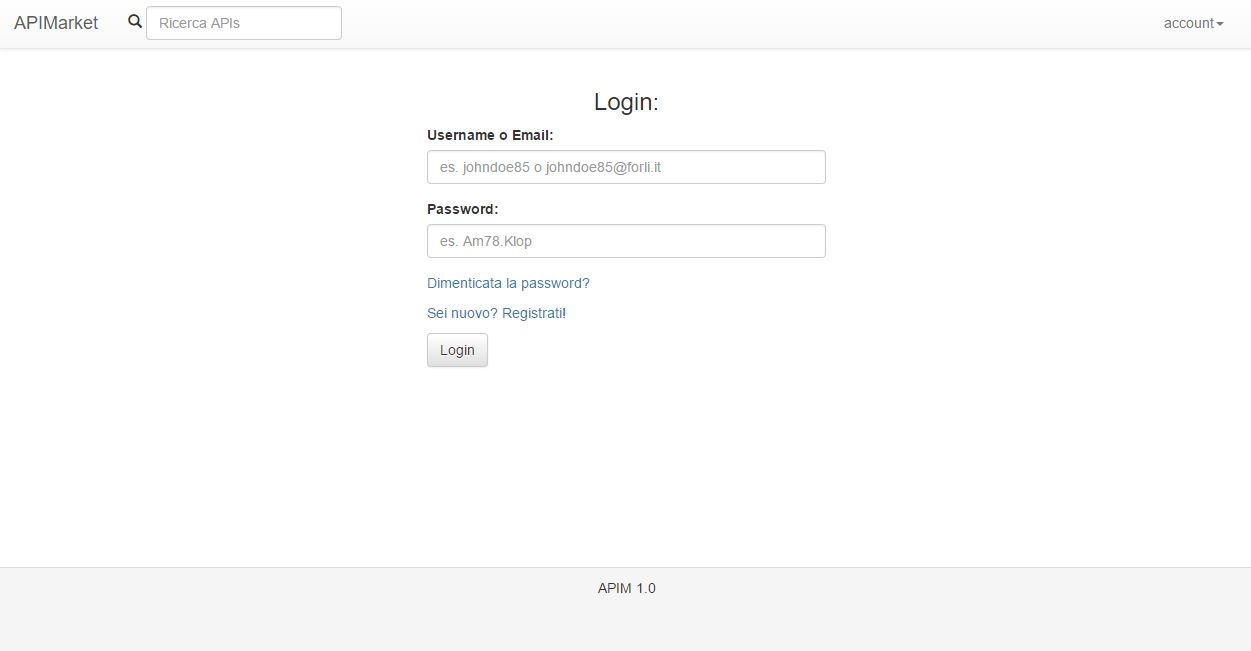
\includegraphics[scale=0.31]{img/APIM_login.JPG}}
		\caption{Login amministratore}
	\end{figure}

\subsection{Pannello amministratore}
	L'ammistratore entrerà in un pannello, dove sulla sinistra può scegliere cose moderare.
	
		\label{Pannello amministratore}
	\begin{figure}[H]
		\centering
		\fbox{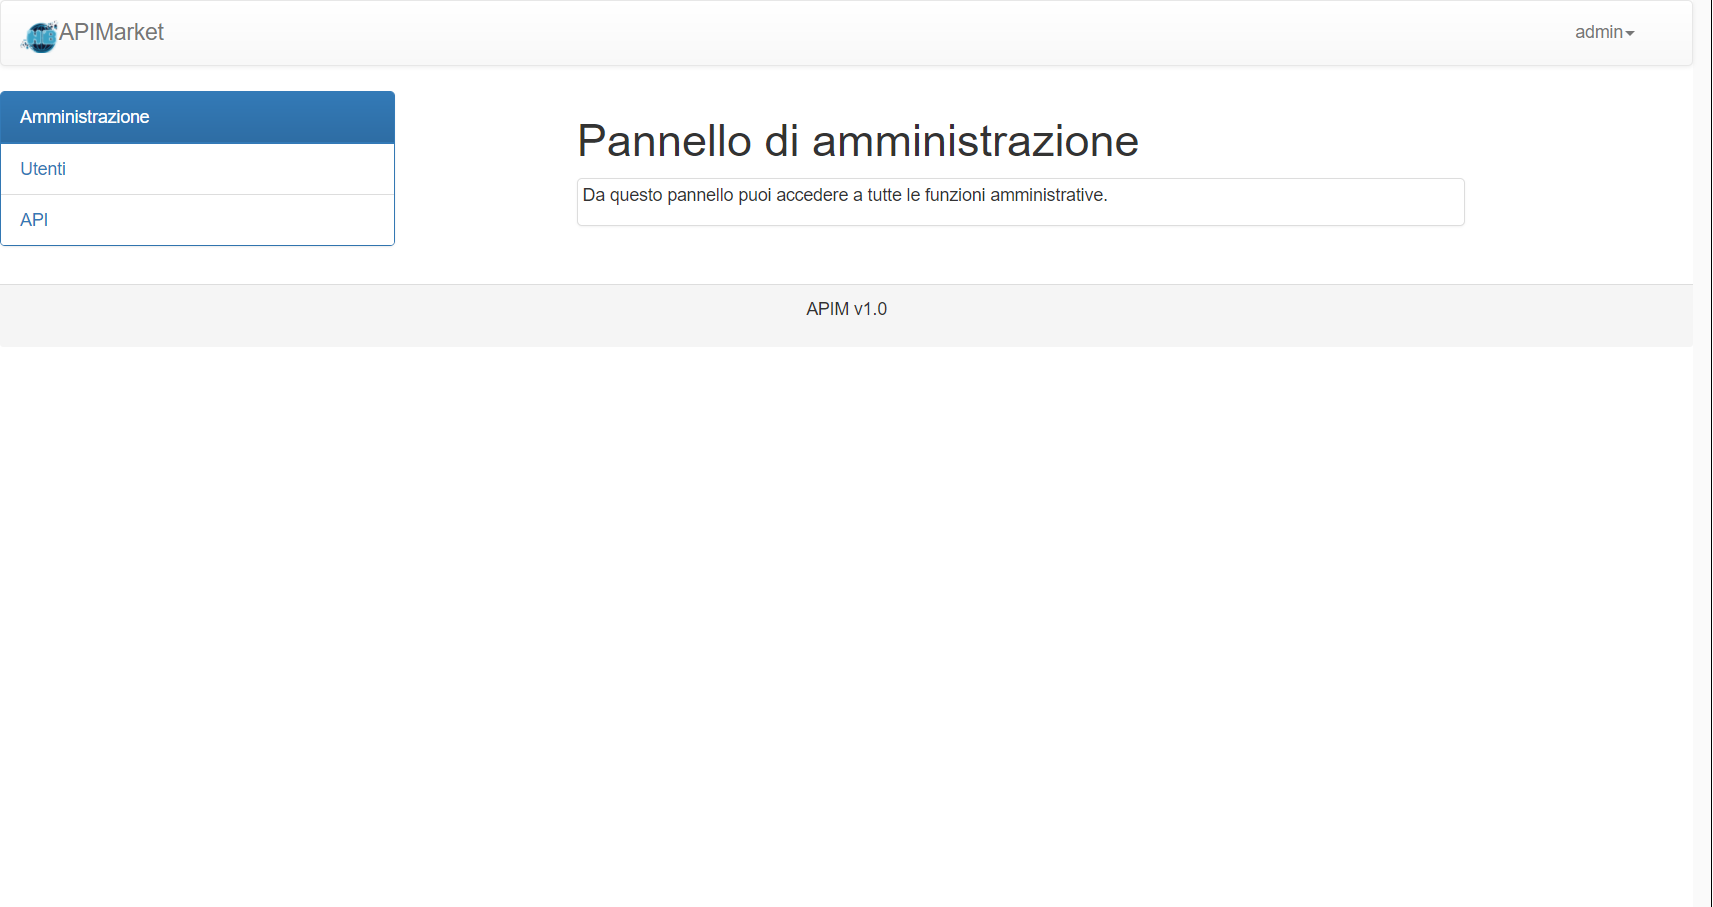
\includegraphics[scale=0.25]{img/APIM_pannelloAdmin.png}}
		\caption{Pannello amministratore}
	\end{figure}
	
	
\subsection{Moderazione API}
Selezionando la voce API, l'amministratore potrà intervenire su tutte le API presenti sul market. Le operazioni possibili sono la sospensione, attivazione e cancellazione di una API, come mostrato di seguito.

	\label{Moderazione API}
	\begin{figure}[H]
		\centering
		\fbox{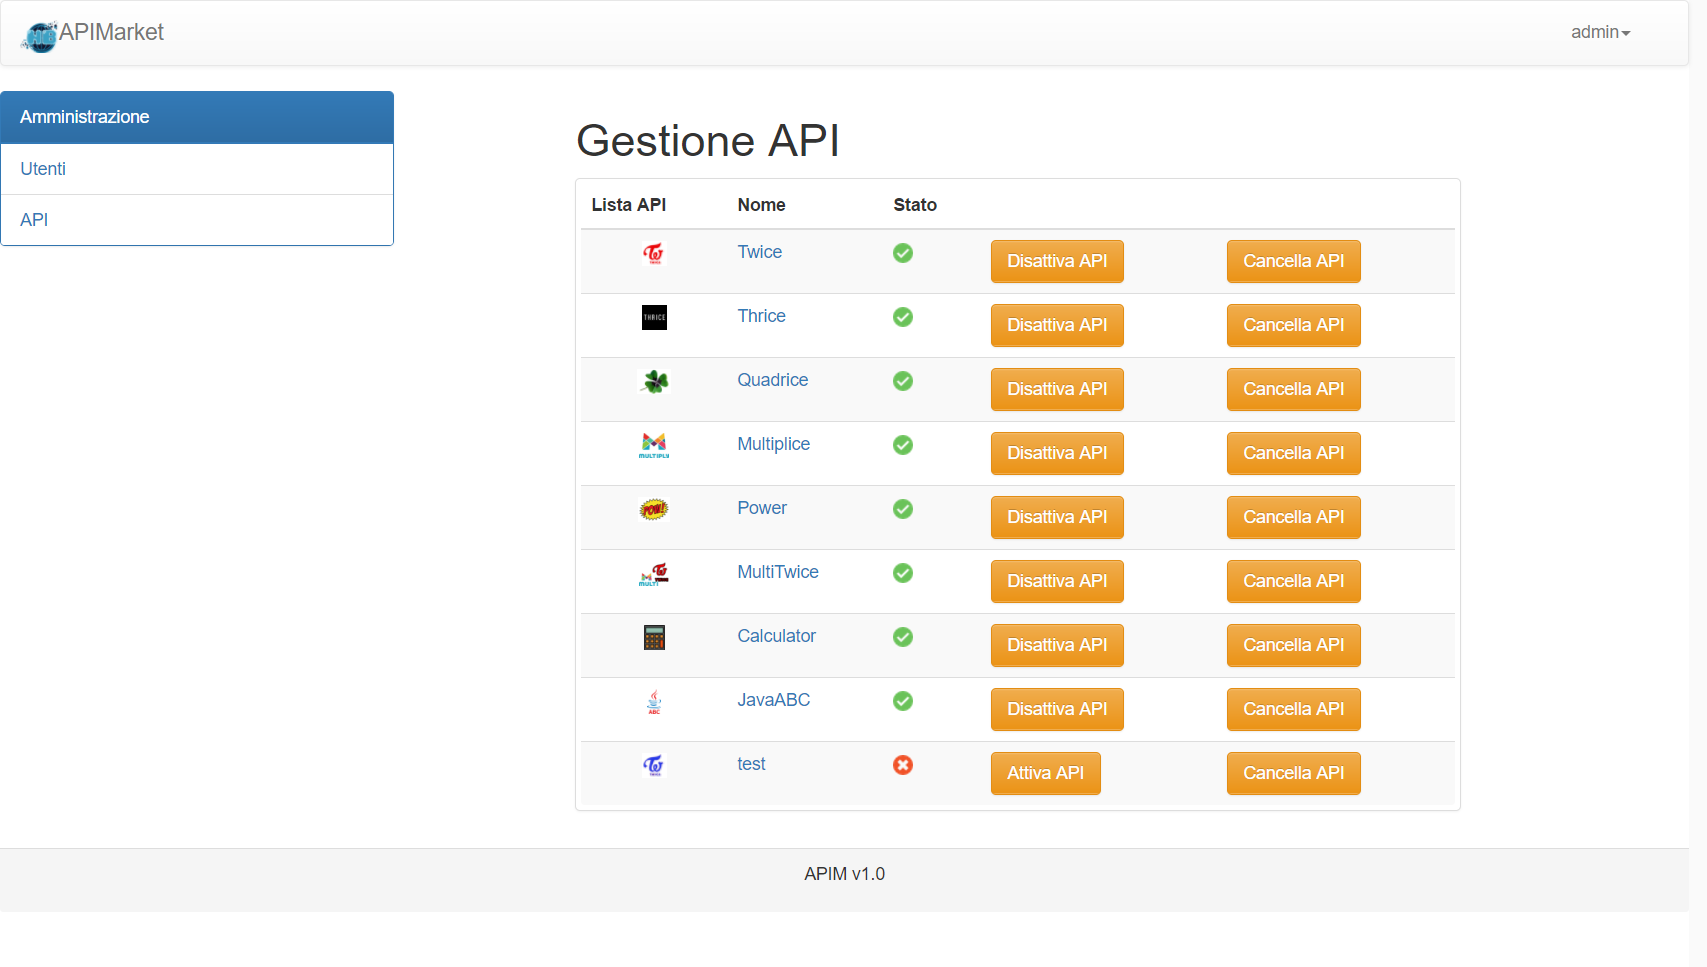
\includegraphics[scale=0.25]{img/APIM_modificaAPI.png}}
		\caption{Moderazione API}
	\end{figure}


\subsection{Moderazione Utente}
Selezionando la voce Utenti, l'amministratore potrà visualizzare le API registrate e attive di tutti gli utenti, con la possibilità di eliminare gli utenti, come mostrato nella seguente immagine.

\label{Moderazione Utente}
\begin{figure}[H]
	\centering
	\fbox{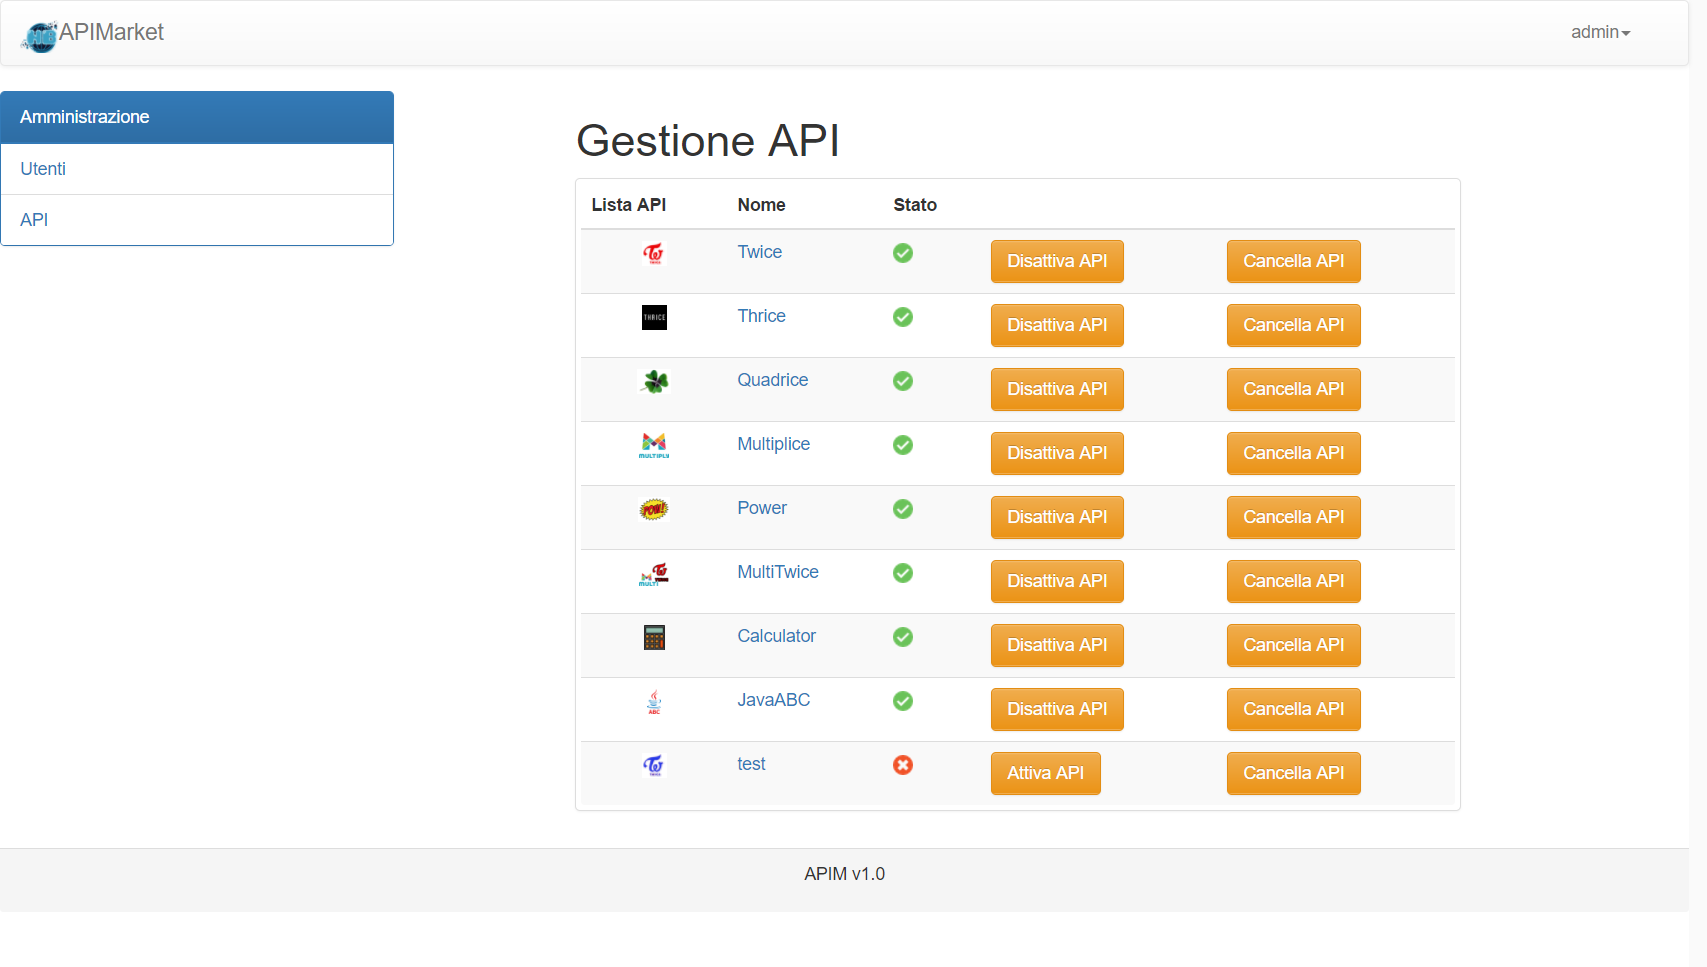
\includegraphics[scale=0.25]{img/APIM_modificaAPI.png}}
	\caption{Moderazione Utente}
\end{figure}
